\documentclass{article}
\usepackage{geometry}
 \geometry{
 a4paper,
 total={170mm,270mm},
 left=20mm,
 top=10mm,
 }
\usepackage{graphicx}
\usepackage{float}
\usepackage{enumitem}
\usepackage{caption}
\usepackage{amsmath}
\usepackage{datetime}
\usepackage{multirow}
\newcommand*{\addheight}[2][.5ex]{%
  \raisebox{0pt}[\dimexpr\height+(#1)\relax]{#2}%
}
\newdate{date}{09}{09}{2016}
\date{\displaydate{date}}
\title{\textbf{Machine Learning - CSCI 5622} \\
HW 2 - LogReg}
\author{\textbf{Santhanakrishnan Ramani}}
\begin{document}
\maketitle

\section*{Analysis}

\begin{enumerate}
\item
How did the learning rate affect the convergence of your SGA implementation?

The figure below shows the graphs of iteration vs training set log probability for different values of eta. We can see clearly that when eta value is very low the rate of convergence is slow, and when eta value is large it diverges and has a very low log probability. So the optimum value for eta will be somewhere near 0.1. 
\begin{table}[H]
\centering
\begin{tabular}{|c|c|c|}
	\hline
	\addheight{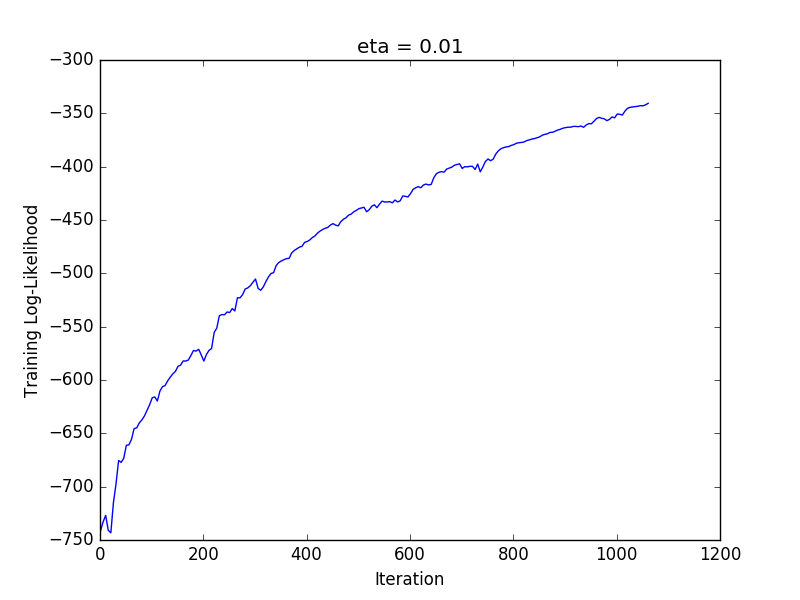
\includegraphics[width=70mm]{images/pointNotOne.png}} &
	\addheight{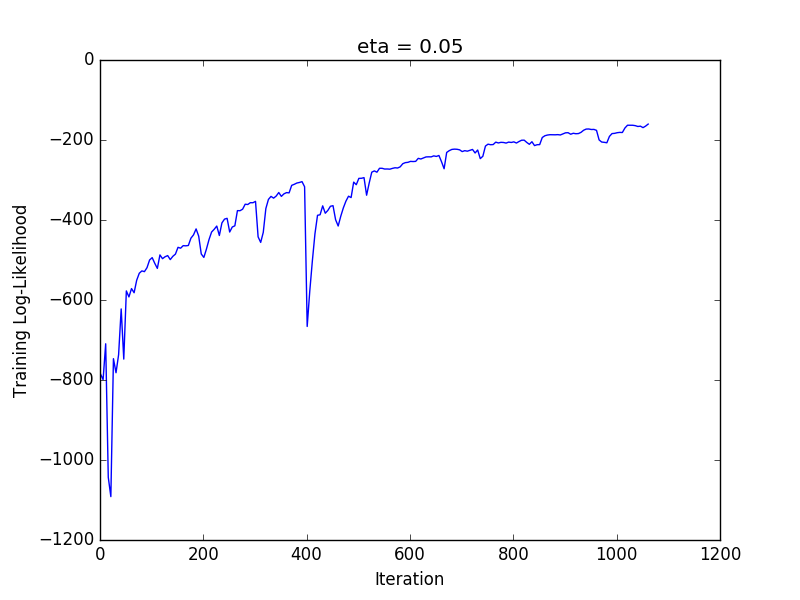
\includegraphics[width=70mm]{images/pointNotFive.png}} \\
	\hline \\    
    \addheight{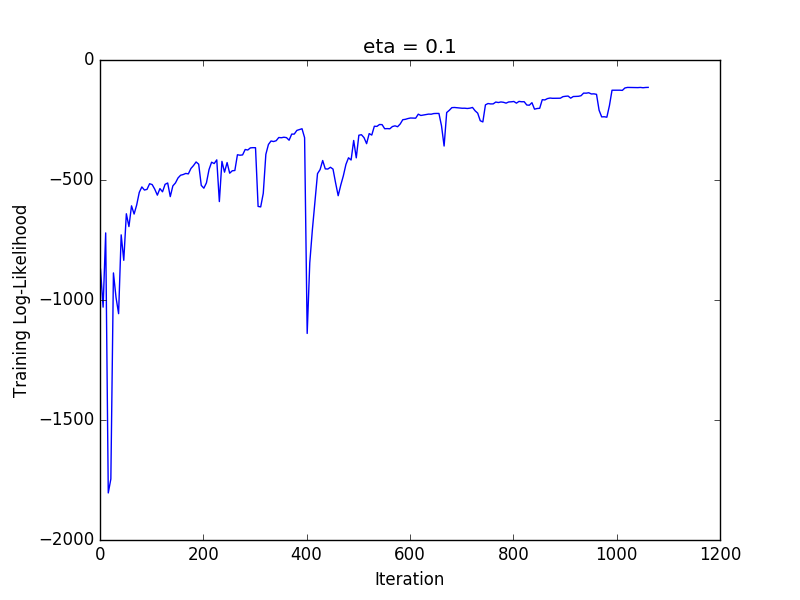
\includegraphics[width=70mm]{images/pointOne.png}} &
    \addheight{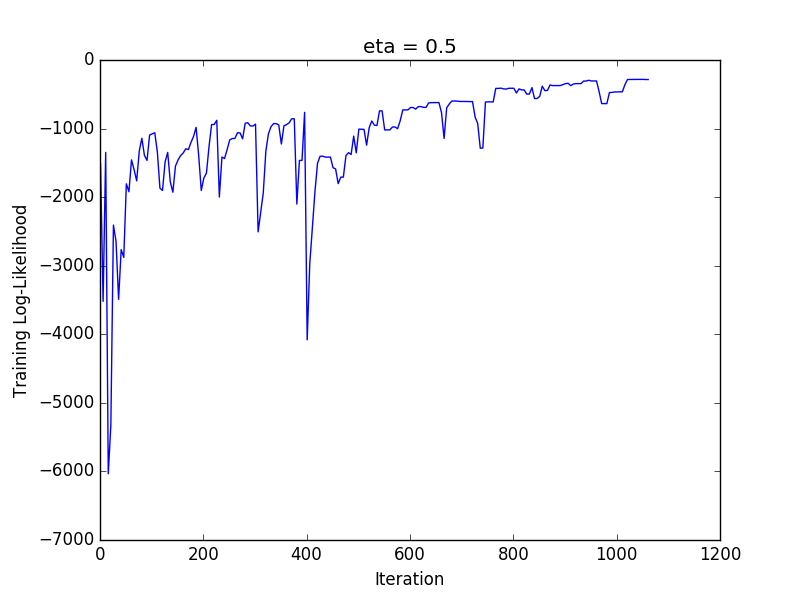
\includegraphics[width=70mm]{images/pointFive.png}} \\
    \hline \\
    \addheight{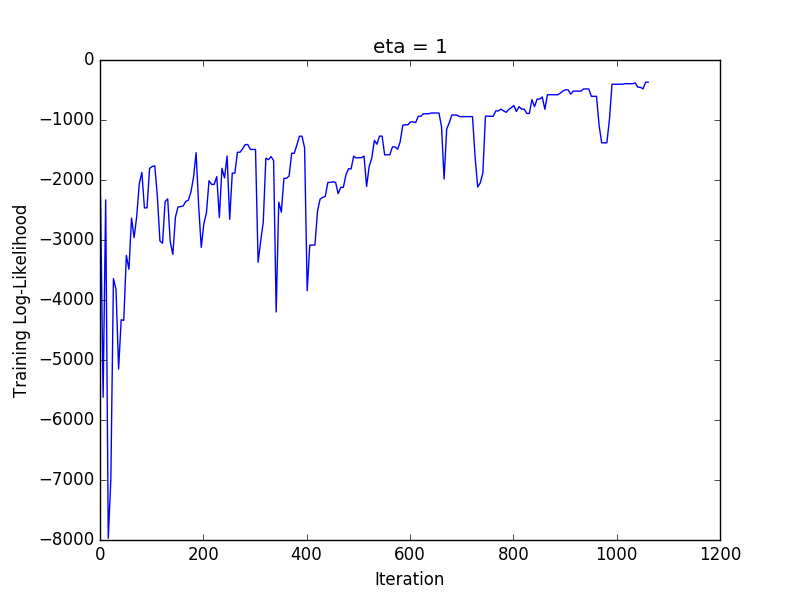
\includegraphics[width=70mm]{images/One.png}} &
    \addheight{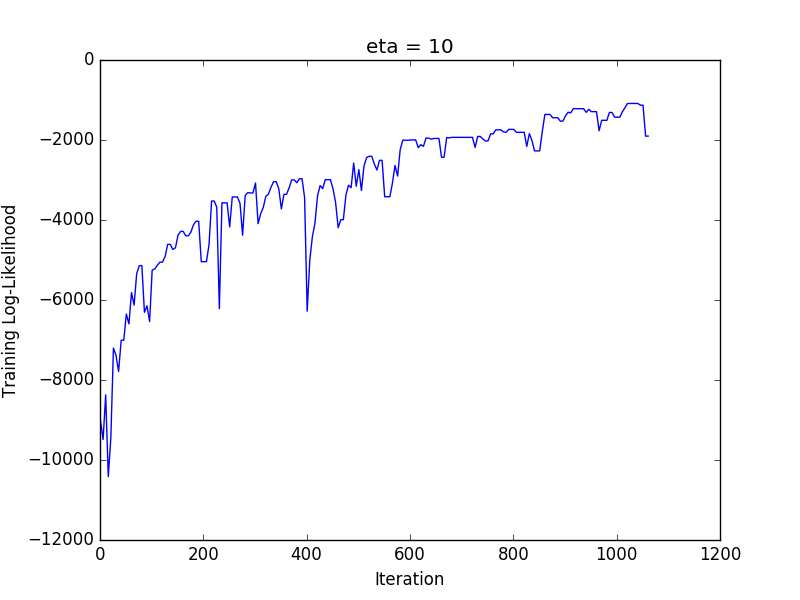
\includegraphics[width=70mm]{images/Ten.png}} \\
    \hline
\end{tabular}
\end{table}
\item
What was your stopping criterion and how many passes over the data did you need to complete before stopping? \\

From the below table we can see the Holdout Accuracy increases until pass 8, then decreases. The stopping criteria is when the Holdout Accuracy stops increasing. The number of passes completed before stopping is 8.
\begin{figure}[!h]
  \centering
  \begin{minipage}[b]{0.8\textwidth}
    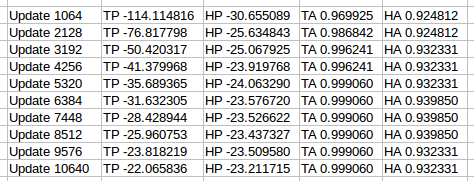
\includegraphics[width=\textwidth]{images/SC.png}
  \end{minipage}
\end{figure}

\item
What words are the best predictors of each class? How (mathematically) did you find them?
\begin{itemize}
\item
Best Predictors for Baseball: pitch, rotation, day, saves, run, baseball,hit
\item
Best Predictors for Hockey: pts, hockey, period, vs, shots, playoff, ice, broadcast \\

I choose words with high positive weights for Baseball, and high negative weights for Hockey.
\end{itemize}

\item
What words are the poorest predictors of classes? How (mathematically) did you find them?
\begin{itemize}
\item
Worst predictors for both classes:\\ contained, sportscasters, favour, prototypical, aggravatingly, pronunciation, crumbled, ratio, baby \\

I chose the words that have either 0 or near 0 weights.
\end{itemize}
\end{enumerate}

\section*{Extra Credit}

\begin{enumerate}
\item
Using a schedule to update the learning rate and its effect.\\
(use the argument --schedule 1 to use eta\_schedule function)\bigskip 

The figure below shows the plot of Iteration vs Training Log Likelihood while using constant eta and a eta schedule. It's clear from the graph that while using a eta schedule the convergence is faster and smoother.

\begin{figure}[h]
  \centering
  \begin{minipage}[b]{0.6\textwidth}
    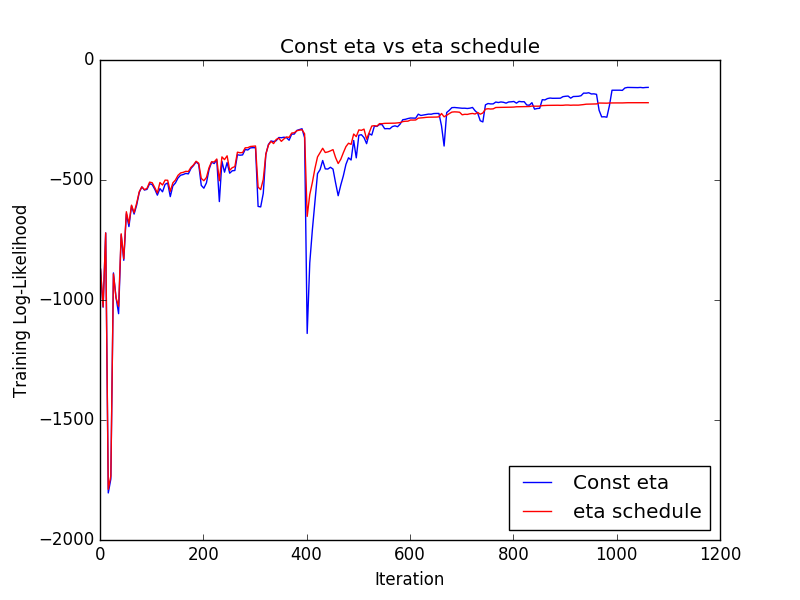
\includegraphics[width=\textwidth]{images/eta.png}
  \end{minipage}
\end{figure}

\item 
Using document frequency to modify the feature values to tf-idf and its effect.\\
(use the argument --tfidf 1 to use ti-idf values)

From the figure below we can see that while using tf-idf the Holdout Accuracy kind of remains constant.

\begin{figure}[h]
  \centering
  \begin{minipage}[b]{0.6\textwidth}
    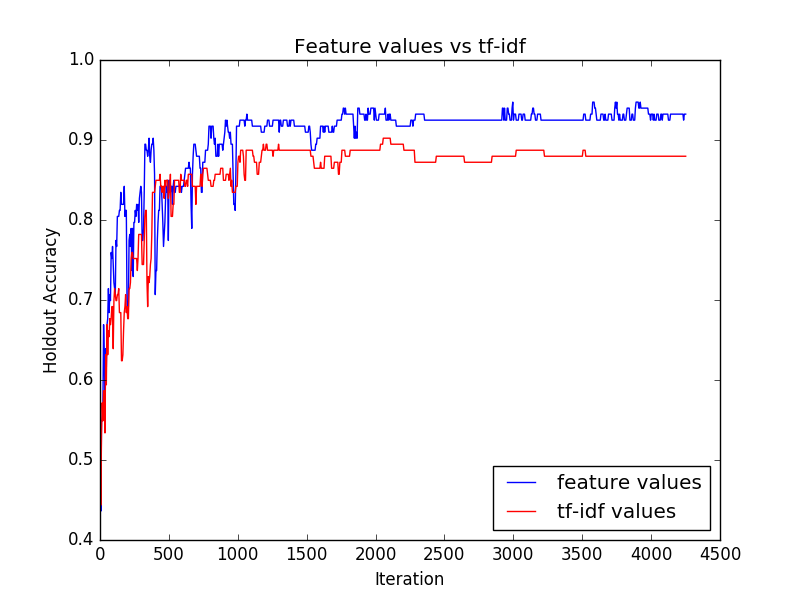
\includegraphics[width=\textwidth]{images/tfidf.png}
  \end{minipage}
\end{figure}

Accuracy of Holdout data when using feature values - 0.924812\\
Accuracy of Holdout data when using  tf-idf  values - 0.887218 \\

So in this problem using tf-idf instead of feature values doesn't improve the accuracy of classification.
\end{enumerate}
\end{document}
